% Created by tikzDevice version 0.12.6 on 2026-05-14 21:28:27
% !TEX encoding = UTF-8 Unicode
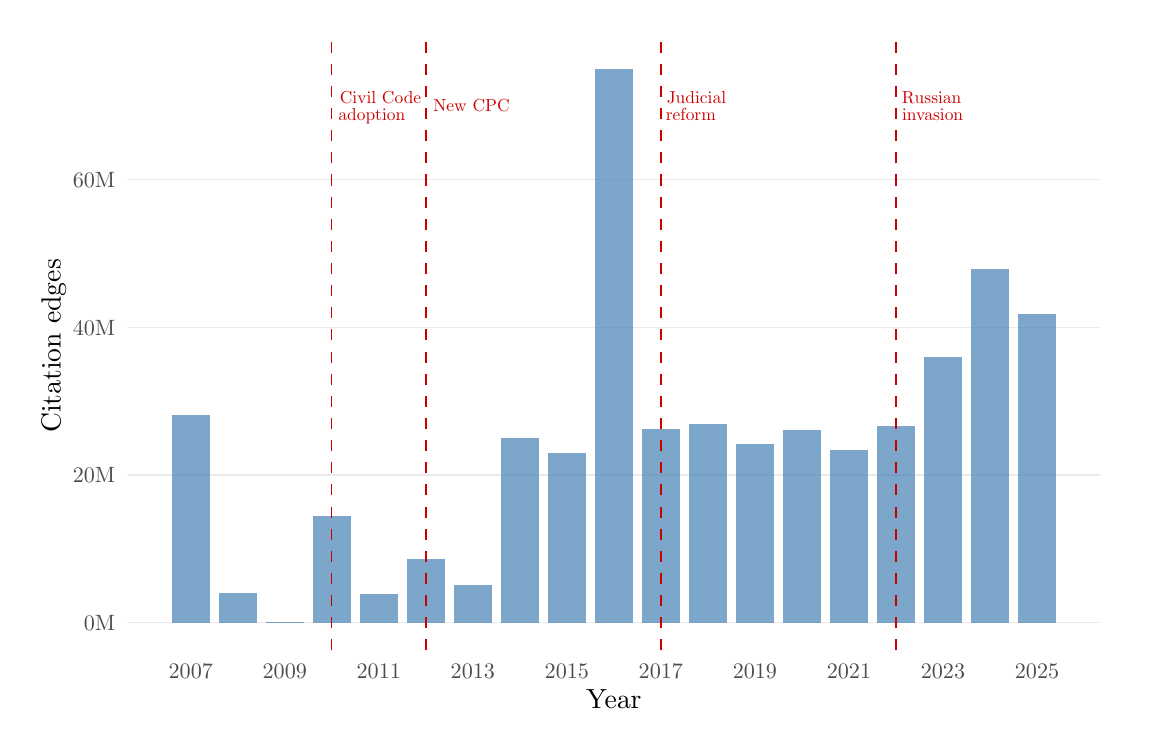
\begin{tikzpicture}[x=1pt,y=1pt]
\definecolor{fillColor}{RGB}{255,255,255}
\path[use as bounding box,fill=fillColor,fill opacity=0.00] (0,0) rectangle (397.48,252.94);
\begin{scope}
\path[clip] (  0.00,  0.00) rectangle (397.48,252.94);
\definecolor{fillColor}{RGB}{255,255,255}

\path[fill=fillColor] ( -0.00,  0.00) rectangle (397.48,252.94);
\end{scope}
\begin{scope}
\path[clip] ( 36.16, 27.90) rectangle (387.48,247.95);
\definecolor{drawColor}{gray}{0.92}

\path[draw=drawColor,line width= 0.5pt,line join=round] ( 36.16, 37.90) --
	(387.48, 37.90);

\path[draw=drawColor,line width= 0.5pt,line join=round] ( 36.16, 91.26) --
	(387.48, 91.26);

\path[draw=drawColor,line width= 0.5pt,line join=round] ( 36.16,144.62) --
	(387.48,144.62);

\path[draw=drawColor,line width= 0.5pt,line join=round] ( 36.16,197.98) --
	(387.48,197.98);
\definecolor{fillColor}{RGB}{70,130,180}

\path[fill=fillColor,fill opacity=0.70] ( 52.13, 37.90) rectangle ( 65.72,113.00);

\path[fill=fillColor,fill opacity=0.70] ( 69.12, 37.90) rectangle ( 82.71, 48.80);

\path[fill=fillColor,fill opacity=0.70] ( 86.11, 37.90) rectangle ( 99.70, 38.22);

\path[fill=fillColor,fill opacity=0.70] (103.10, 37.90) rectangle (116.69, 76.39);

\path[fill=fillColor,fill opacity=0.70] (120.08, 37.90) rectangle (133.68, 48.46);

\path[fill=fillColor,fill opacity=0.70] (137.07, 37.90) rectangle (150.66, 61.06);

\path[fill=fillColor,fill opacity=0.70] (154.06, 37.90) rectangle (167.65, 51.70);

\path[fill=fillColor,fill opacity=0.70] (171.05, 37.90) rectangle (184.64,104.52);

\path[fill=fillColor,fill opacity=0.70] (188.04, 37.90) rectangle (201.63, 99.40);

\path[fill=fillColor,fill opacity=0.70] (205.03, 37.90) rectangle (218.62,237.94);

\path[fill=fillColor,fill opacity=0.70] (222.02, 37.90) rectangle (235.61,108.00);

\path[fill=fillColor,fill opacity=0.70] (239.00, 37.90) rectangle (252.60,109.84);

\path[fill=fillColor,fill opacity=0.70] (255.99, 37.90) rectangle (269.58,102.57);

\path[fill=fillColor,fill opacity=0.70] (272.98, 37.90) rectangle (286.57,107.66);

\path[fill=fillColor,fill opacity=0.70] (289.97, 37.90) rectangle (303.56,100.32);

\path[fill=fillColor,fill opacity=0.70] (306.96, 37.90) rectangle (320.55,108.96);

\path[fill=fillColor,fill opacity=0.70] (323.95, 37.90) rectangle (337.54,134.02);

\path[fill=fillColor,fill opacity=0.70] (340.94, 37.90) rectangle (354.53,165.58);

\path[fill=fillColor,fill opacity=0.70] (357.92, 37.90) rectangle (371.52,149.58);
\definecolor{drawColor}{RGB}{205,0,0}

\path[draw=drawColor,line width= 0.5pt,dash pattern=on 4pt off 4pt ,line join=round] (109.89, 27.90) -- (109.89,247.95);

\path[draw=drawColor,line width= 0.5pt,dash pattern=on 4pt off 4pt ,line join=round] (143.87, 27.90) -- (143.87,247.95);

\path[draw=drawColor,line width= 0.5pt,dash pattern=on 4pt off 4pt ,line join=round] (228.81, 27.90) -- (228.81,247.95);

\path[draw=drawColor,line width= 0.5pt,dash pattern=on 4pt off 4pt ,line join=round] (313.75, 27.90) -- (313.75,247.95);

\node[text=drawColor,anchor=base west,inner sep=0pt, outer sep=0pt, scale=  0.63] at (112.81,225.69) {Civil Code};

\node[text=drawColor,anchor=base west,inner sep=0pt, outer sep=0pt, scale=  0.63] at (112.29,219.31) {adoption};

\node[text=drawColor,anchor=base west,inner sep=0pt, outer sep=0pt, scale=  0.63] at (146.61,222.50) {New CPC};

\node[text=drawColor,anchor=base west,inner sep=0pt, outer sep=0pt, scale=  0.63] at (230.94,225.69) {Judicial};

\node[text=drawColor,anchor=base west,inner sep=0pt, outer sep=0pt, scale=  0.63] at (230.61,219.31) {reform};

\node[text=drawColor,anchor=base west,inner sep=0pt, outer sep=0pt, scale=  0.63] at (315.89,225.69) {Russian};

\node[text=drawColor,anchor=base west,inner sep=0pt, outer sep=0pt, scale=  0.63] at (315.95,219.31) {invasion};
\end{scope}
\begin{scope}
\path[clip] (  0.00,  0.00) rectangle (397.48,252.94);
\definecolor{drawColor}{gray}{0.30}

\node[text=drawColor,anchor=base east,inner sep=0pt, outer sep=0pt, scale=  0.80] at ( 31.66, 35.14) {0M};

\node[text=drawColor,anchor=base east,inner sep=0pt, outer sep=0pt, scale=  0.80] at ( 31.66, 88.50) {20M};

\node[text=drawColor,anchor=base east,inner sep=0pt, outer sep=0pt, scale=  0.80] at ( 31.66,141.86) {40M};

\node[text=drawColor,anchor=base east,inner sep=0pt, outer sep=0pt, scale=  0.80] at ( 31.66,195.22) {60M};
\end{scope}
\begin{scope}
\path[clip] (  0.00,  0.00) rectangle (397.48,252.94);
\definecolor{drawColor}{gray}{0.30}

\node[text=drawColor,anchor=base,inner sep=0pt, outer sep=0pt, scale=  0.80] at ( 58.93, 17.89) {2007};

\node[text=drawColor,anchor=base,inner sep=0pt, outer sep=0pt, scale=  0.80] at ( 92.90, 17.89) {2009};

\node[text=drawColor,anchor=base,inner sep=0pt, outer sep=0pt, scale=  0.80] at (126.88, 17.89) {2011};

\node[text=drawColor,anchor=base,inner sep=0pt, outer sep=0pt, scale=  0.80] at (160.86, 17.89) {2013};

\node[text=drawColor,anchor=base,inner sep=0pt, outer sep=0pt, scale=  0.80] at (194.83, 17.89) {2015};

\node[text=drawColor,anchor=base,inner sep=0pt, outer sep=0pt, scale=  0.80] at (228.81, 17.89) {2017};

\node[text=drawColor,anchor=base,inner sep=0pt, outer sep=0pt, scale=  0.80] at (262.79, 17.89) {2019};

\node[text=drawColor,anchor=base,inner sep=0pt, outer sep=0pt, scale=  0.80] at (296.77, 17.89) {2021};

\node[text=drawColor,anchor=base,inner sep=0pt, outer sep=0pt, scale=  0.80] at (330.74, 17.89) {2023};

\node[text=drawColor,anchor=base,inner sep=0pt, outer sep=0pt, scale=  0.80] at (364.72, 17.89) {2025};
\end{scope}
\begin{scope}
\path[clip] (  0.00,  0.00) rectangle (397.48,252.94);
\definecolor{drawColor}{RGB}{0,0,0}

\node[text=drawColor,anchor=base,inner sep=0pt, outer sep=0pt, scale=  1.00] at (211.82,  6.94) {Year};
\end{scope}
\begin{scope}
\path[clip] (  0.00,  0.00) rectangle (397.48,252.94);
\definecolor{drawColor}{RGB}{0,0,0}

\node[text=drawColor,rotate= 90.00,anchor=base,inner sep=0pt, outer sep=0pt, scale=  1.00] at ( 11.89,137.92) {Citation edges};
\end{scope}
\end{tikzpicture}
